% =========================================================================
% DocMind Technical Report — LaTeX source
% Target venue: arXiv (cs.IR / cs.CL) — single-column article layout
% Build: pdflatex main && bibtex main && pdflatex main && pdflatex main
% =========================================================================
\documentclass[11pt,a4paper]{article}

\usepackage[T1]{fontenc}
\usepackage[utf8]{inputenc}
\usepackage{lmodern}
\usepackage{microtype}
\usepackage[margin=2.6cm]{geometry}
\usepackage{graphicx}
\usepackage{booktabs}
\usepackage{amsmath}
\usepackage[hidelinks]{hyperref}
\usepackage{url}
\usepackage[numbers,sort&compress]{natbib}
\usepackage{caption}
\captionsetup{font=small,labelfont=bf}

\graphicspath{{assets/}}

\newcommand{\ie}{i.e.}
\newcommand{\eg}{e.g.}

\title{\bfseries DocMind: A Self-Hosted Retrieval-Augmented Generation Platform
with Measurable Retrieval Quality, Deterministic Layered Caching, and
Operations-Grade Governance}

\author{Yuxiuquan \\ \small Independent project report --- source code available from the author}
\date{August 30, 2026}

\begin{document}
\maketitle

\begin{abstract}
Retrieval-augmented generation (RAG) systems are usually demonstrated rather than
measured: prototypes are wired to a vector store and a prompt, but provide no answer
to how much a design change helps, which queries are silently dropped, or what a
system costs to run. This report describes DocMind, a self-hosted multi-assistant RAG
platform built around three engineering commitments. First, retrieval quality is
\emph{measured}: a fixed 47-question benchmark (30 canonical, 17 adversarially
colloquial) gates every change, showing that hybrid BM25--dense fusion via reciprocal
rank fusion (RRF) lifts adversarial Recall@4 from 94.1\% to 100.0\%, while
cross-encoder reranking improves MRR by 7.8\% at a deliberate one-hit recall cost
imposed by threshold filtering. Second, cost and latency are \emph{engineered}, not
hoped for: a four-layer cache hierarchy keyed by determinism (tokenizer, document
embeddings, query embeddings, and rerank results) removes all upstream API
round-trips for repeated questions --- throughput on a warm replayed-question workload
rises from 3.1 to 801 QPS with P95 latency dropping from 2{,}573\,ms to 11\,ms, while
cold queries show no regression. Third, fine-tuning is applied \emph{narrowly}: a
rank-8 LoRA adapter tuned on a 1.5B model rewrites colloquial queries before
retrieval, improving overall Recall@4 by 3.97 points at zero marginal API cost; a
controlled experiment attributes the remaining headroom to corpus coverage rather than
rewriting quality. The platform further integrates evidence-grounded refusal,
RAGAS-style generation metrics, document-level access control, an MCP server surface,
and full audit and alerting, and is deployed as a single docker-compose stack behind
an nginx entry point.

\medskip
\noindent\textbf{Keywords:} retrieval-augmented generation; hybrid retrieval;
reciprocal rank fusion; cross-encoder reranking; LoRA; query rewriting; caching;
evaluation; self-hosting
\end{abstract}

% ---------------------------------------------------------------------
\section{Introduction}\label{sec:intro}

Production LLM applications in the retrieval-augmented generation (RAG) style are now
straightforward to prototype: embed a corpus, retrieve top-$k$, and prompt a chat
model. The hard part begins after the demo. Teams cannot answer basic questions ---
which fraction of user queries fails silently, how a chunking change affects recall,
what a month of traffic costs, or whether an answer is grounded in retrieved evidence.
We call this gap the difference between a \emph{RAG demo} and a \emph{RAG system}, and
we built DocMind to close it.

DocMind is a self-hosted, multi-assistant, multi-knowledge-base platform. Its retrieval
pipeline is hybrid (BM25 plus dense vectors fused by reciprocal rank fusion, followed
by a cross-encoder reranker); its agent is a hand-written ReAct loop with an
evidence-grounded refusal path; and its operation is wrapped in an evaluation harness,
cost accounting, alerting, and audit logging. The design philosophy is deliberately
conservative: every enhancement component must degrade gracefully and must never block
the answering path, and every claimed improvement must come with a reproducible number
from a fixed benchmark.

This report makes four concrete contributions.
\begin{enumerate}
  \item A benchmark-driven comparison of three retrieval routes on canonical and
        adversarially colloquial question sets, with an analysis of why rerank
        thresholds trade recall for refusal safety (Section~\ref{sec:retrieval}).
  \item A four-layer cache hierarchy organized by the determinism of each cached
        function, with an A/B evaluation on identical code showing a $258\times$
        throughput improvement on warm replayed-question workloads and zero regression
        on cold queries (Section~\ref{sec:cache}).
  \item A narrow-task fine-tuning study: a LoRA-adapted 1.5B query rewriter with
        deterministic training-data construction, plus a controlled experiment that
        separates rewriting quality from corpus coverage (Section~\ref{sec:lora}).
  \item An operations-grade governance layer --- audit, alerting, backup, access
        control, and an MCP tool surface --- that makes the platform deployable inside
        organizations (Section~\ref{sec:governance}).
\end{enumerate}

% ---------------------------------------------------------------------
\section{System Overview}\label{sec:overview}

Figure~\ref{fig:arch} shows the deployment topology. A single nginx process serves the
React single-page application and reverse-proxies REST and server-sent-event (SSE)
traffic to a FastAPI host; the whole stack ships as one docker-compose project behind
ports 80/443. The application host embeds a hand-written ReAct agent --- no agent
framework --- with a tool registry exposing knowledge retrieval, web search with a
four-engine fallback chain, and MCP tools. Authentication supports local accounts
(PBKDF2 with per-user salt), forced first-login password rotation, and optional
enterprise LDAP. Document-level access control is enforced inside the retrieval
pipeline itself: unauthorized documents are filtered \emph{before} truncation so that
restricted content neither leaks nor crowds out authorized candidates.

\begin{figure}[t]
  \centering
  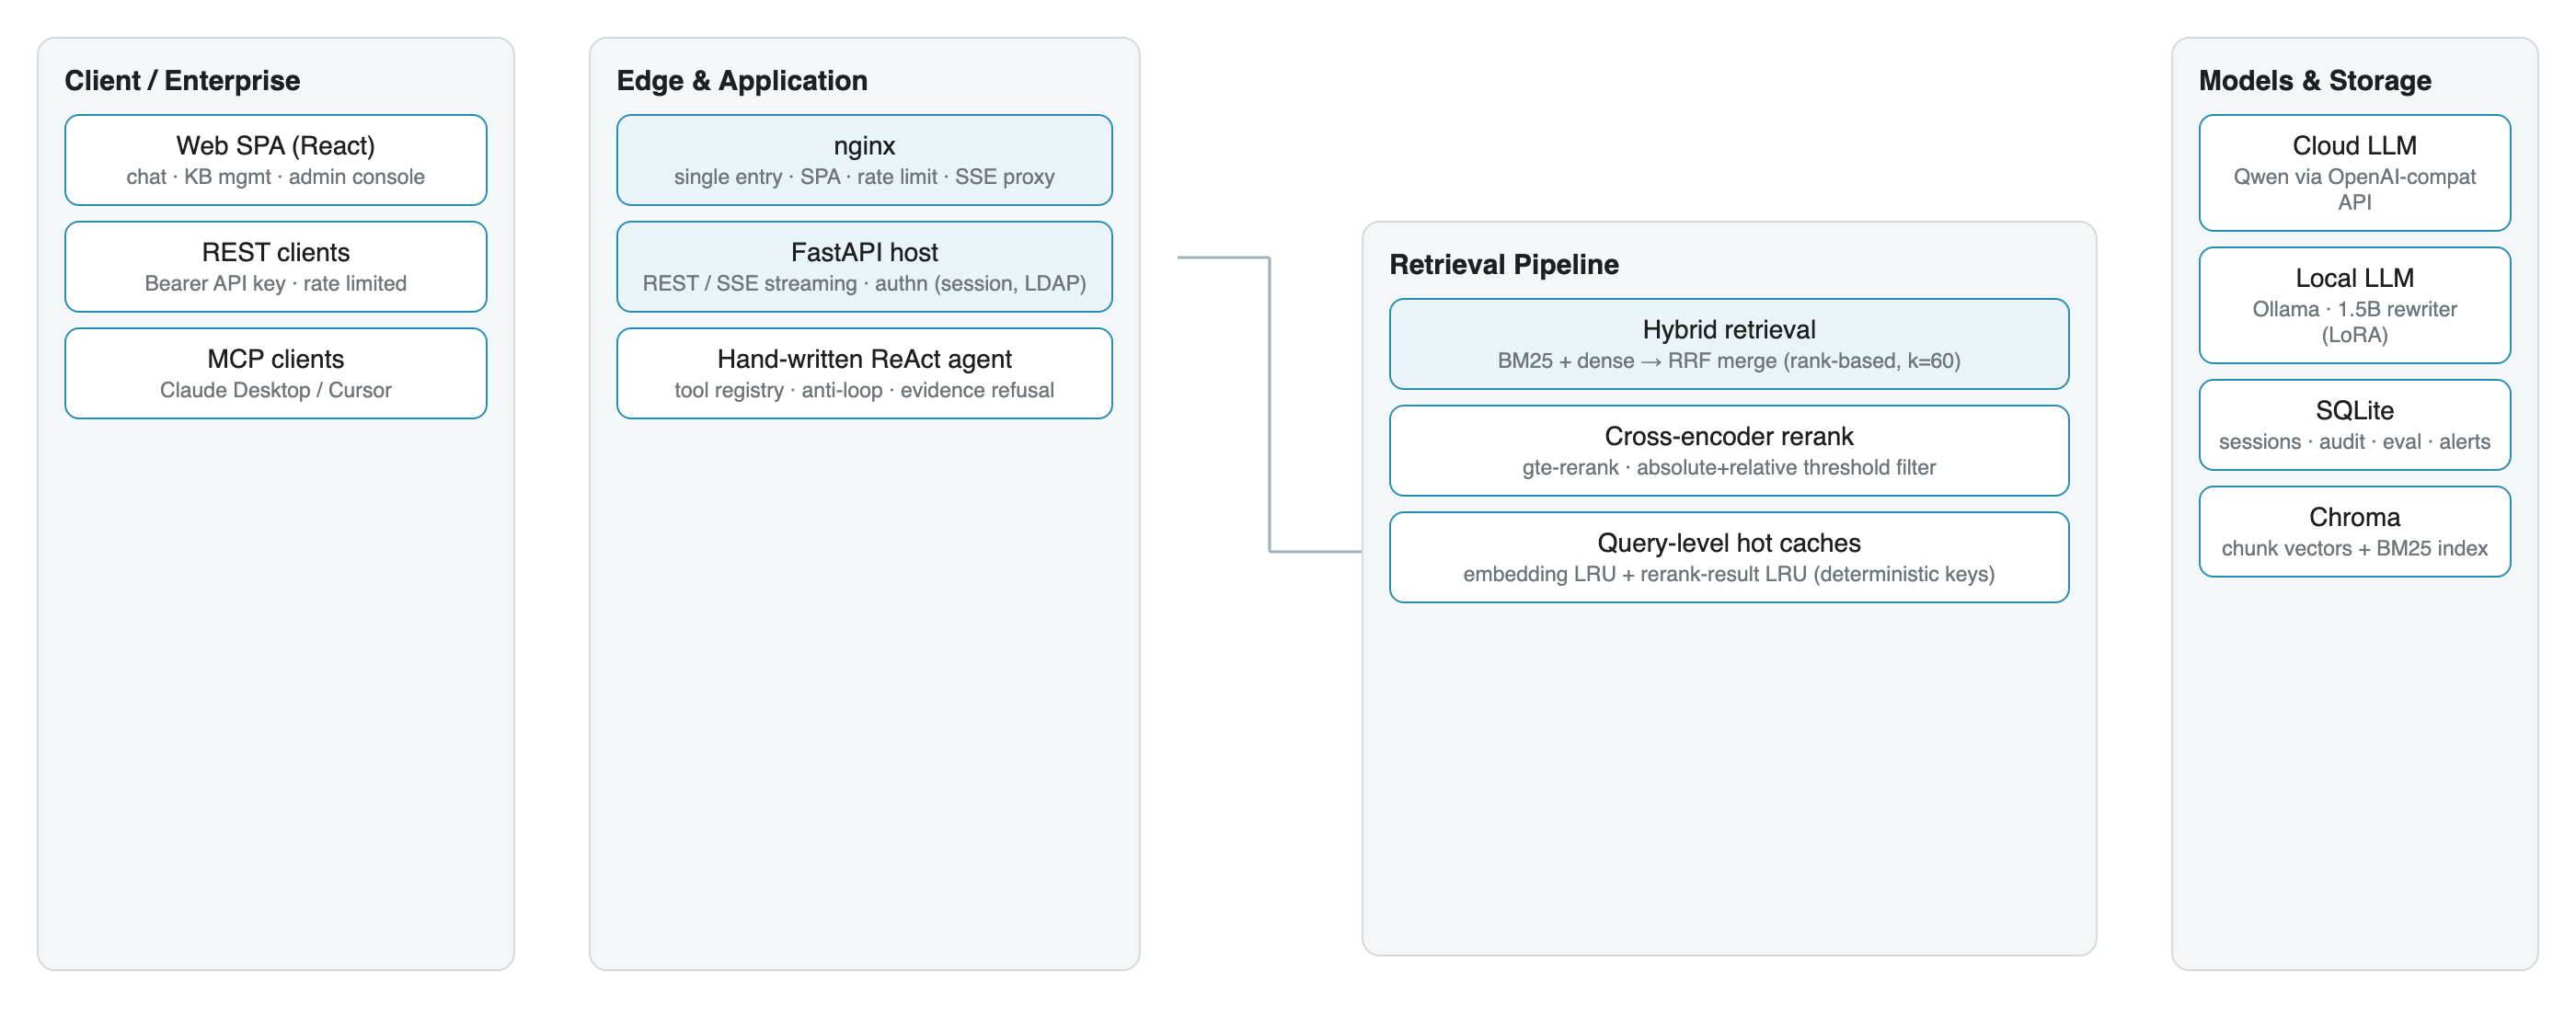
\includegraphics[width=\textwidth]{arch.png}
  \caption{DocMind deployment and data flow. Enhancements (reranker, caches, web
  search) degrade gracefully; the answering path never depends on them succeeding.}
  \label{fig:arch}
\end{figure}

Two principles shaped the implementation. First, the agent core is owned code: the
ReAct loop, tool-result sanitization, injection guards, and the anti-dead-loop budget
are implemented in-tree, which keeps the trust boundary explicit and the behavior
auditable. Second, every enhancement is optional at runtime: the reranker falls back to
RRF ordering on failure, Langfuse falls back to local JSONL tracing, and web search
falls back across four providers. Degradation is a design decision, not an incident.

% ---------------------------------------------------------------------
\section{Hybrid Retrieval and the Cost of Thresholds}\label{sec:retrieval}

The retrieval pipeline runs two parallel recall paths --- a BM25 lexical path over
jieba-tokenized chunks and a dense path over Chroma-stored embeddings --- and merges
them with reciprocal rank fusion using $k = 60$~\citep{cormack2009rrf}. RRF is chosen
over score interpolation because BM25 scores are unbounded while cosine similarities
lie in $[0,1]$; rank-based fusion makes the merge invariant to these incompatible
scales and requires no tuning.

Merged candidates are capped at ten and passed to a cross-encoder reranker
(gte-rerank-v2~\citep{gte2023}). Because relevance scores from the reranker are
calibrated probabilities, the pipeline applies a two-part filter: an absolute floor
(0.05, or a 0.08 floor on the top hit, below which the system escalates to refusal) and
a relative filter at 15\% of the head score.

Table~\ref{tab:routes} reports the fixed-benchmark comparison. Three observations
matter. First, canonical questions are essentially saturated by modern embeddings ---
differentiation only appears on the adversarial set, which contains colloquial,
code-mixed, and abbreviation-heavy phrasings. Second, RRF raises adversarial Recall@4
from 94.1\% to 100.0\%: BM25 supplies exactly the literal matching that dense
embeddings miss on jargon. Third, adding the reranker improves MRR from 0.873 to
0.941 --- the correct chunk is ranked markedly higher --- while recall drops by one
borderline hit, which the relative threshold removes. We retain the threshold
deliberately: downstream, the evidence-grounded refusal path prefers an honest ``not in
the knowledge base'' over an answer woven from a weakly related chunk. The trade-off is
explicit, benchmarked, and tunable per deployment.

\begin{table}[t]
  \centering
  \caption{Retrieval routes on the 47-question benchmark (30 canonical, 17
  adversarial). Every number is produced by the benchmark script and is reproducible
  from the repository.}
  \label{tab:routes}
  \begin{tabular}{lcc}
    \toprule
    Route & Recall@4 (canon.\ / adv.) & MRR (canon.\ / adv.) \\
    \midrule
    Dense only              & 100.0\% / 94.1\%  & 0.978 / 0.843 \\
    Hybrid + RRF            & 100.0\% / 100.0\% & 1.000 / 0.873 \\
    Hybrid + RRF + rerank   & 100.0\% / 94.1\%  & 1.000 / 0.941 \\
    \bottomrule
  \end{tabular}
\end{table}

Two engineering details extend the result to multi-knowledge-base deployments. Recall
paths run per knowledge base without reranking; merged, deduplicated candidates are
then reranked exactly once, cutting reranker API cost by a factor of the base count
while keeping scores comparable across bases. And because the reranker is a remote API,
failures fall back to RRF ordering, with a circuit breaker (three consecutive failures
trigger a 60\,s cooldown) so that endpoint outages degrade ranking quality rather than
availability.

% ---------------------------------------------------------------------
\section{A Determinism-Keyed Cache Hierarchy}\label{sec:cache}

Per-request latency is dominated by two remote calls: one embedding of the query and
one rerank of the candidates. Both are deterministic functions of their inputs for a
fixed model, which makes them safely cacheable at the query level --- the cache changes
\emph{whether} a value is recomputed, never \emph{what} the value is.

DocMind therefore maintains four layers, ordered by where determinism is easiest to
argue: a CPU-level tokenizer cache over unchanged chunks; a persistent SQLite embedding
cache over document chunks (keyed by text hash, invalidated on write failure); an
in-process LRU over query embeddings; and an in-process LRU over rerank results. Cache
keys embed the model name and --- for the rerank cache --- a SHA-256 fingerprint of the
candidate set, so that a model switch or a knowledge-base update changes the key and
old entries expire structurally, with no manual invalidation. Only successful results
are cached, so failure and circuit-breaker semantics are unchanged; notably, hot
queries served from cache remain available even while the breaker is open.

Table~\ref{tab:cache} reports a same-code A/B evaluation on the open retrieval
endpoint. The same 12-question set is replayed at three concurrency levels, and because
the caches persist across passes the first pass is entirely cold --- every question
traverses the full pipeline (12 misses) --- while the second and third passes are
served entirely from cache (24 hits). Replaying a warm question set models the
repeat-query pattern that dominates FAQ-shaped enterprise traffic. Cache toggles are
environment flags, so both runs execute identical code. Warm-pass throughput improves
by roughly two orders of magnitude and P95 collapses from 2{,}573\,ms to 11\,ms; the
cold pass is statistically unchanged, demonstrating that the caches neither help nor
hurt long-tail queries. Hit rates are exported as Prometheus counters (67\%: 12
misses, 24 hits).

\begin{table}[t]
  \centering
  \caption{Same-code A/B with query-level caches toggled by flag: the identical
  12-question set replayed at three concurrency levels. Warm passes skip both upstream
  round-trips; the answer-level semantic cache (similarity-matched, threshold 0.92)
  sits above this layer and is unaffected.}
  \label{tab:cache}
  \begin{tabular}{lcc}
    \toprule
    Scenario & Baseline (QPS / P95) & With caches (QPS / P95) \\
    \midrule
    Concurrency 1 --- first pass, cold  & 2.46 / 1{,}040\,ms & 2.84 / 1{,}059\,ms \\
    Concurrency 4 --- second pass, warm & 2.97 / 1{,}390\,ms & 741 / 6\,ms        \\
    Concurrency 8 --- third pass, warm  & 3.10 / 2{,}573\,ms & 801 / 11\,ms       \\
    \bottomrule
  \end{tabular}
\end{table}

% ---------------------------------------------------------------------
\section{Narrow Fine-Tuning: a LoRA Query Rewriter}\label{sec:lora}

Colloquial phrasings are the weak spot of dense recall. The common fix --- asking the
chat LLM to rewrite each query --- costs one extra cloud round-trip per turn. DocMind
instead fine-tunes a 1.5B model (Qwen2.5-1.5B-Instruct~\citep{qwen25}) as a dedicated
rewriter: a rank-8 LoRA adapter~\citep{hu2022lora} trained with LLaMA-Factory on a
MacBook (about 20 minutes), merged and served locally through Ollama as GGUF. The
rewriter is a bypass component: if it fails or outputs nothing, retrieval proceeds with
the raw query.

Training data is constructed deterministically: the 47 benchmark seed questions are
expanded by fixed-seed noise rules into colloquial, code-mixed, typo, and preamble
variants --- eight per question plus the canonical form --- yielding 364 deduplicated
pairs with a 90/10 train-validation split. The A/B evaluation draws from a disjoint
noise-seed range: three held-out variants per question (141 generated, 126 valid after
deduplication), so no evaluation string appears in the training corpus. Because the
seeds and rules are fixed, any rerun reproduces the identical datasets. On this
evaluation, the tuned rewriter improves overall Recall@4 from 0.754 to 0.794 (+3.97
points) and canonical-group recall from 0.827 to 0.889 (+6.17 points), at a local
rewrite latency of about 400\,ms (Table~\ref{tab:lora}). The rewrite step itself now
costs zero API calls.

\begin{table}[t]
  \centering
  \caption{Recall@4 of retrieval after rewriting, baseline (untuned 1.5B) versus
  LoRA-tuned rewriter, on 126 deterministic samples.}
  \label{tab:lora}
  \begin{tabular}{lccc}
    \toprule
    Group (n) & Baseline rewrite & Tuned rewrite & Delta \\
    \midrule
    Overall (126)    & 0.754 & 0.794 & $+3.97$\,pp \\
    Canonical (81)   & 0.827 & 0.889 & $+6.17$\,pp \\
    Adversarial (45) & 0.622 & 0.622 & $0.00$      \\
    \bottomrule
  \end{tabular}
\end{table}

The adversarial group did not move, and a controlled experiment explains why:
retrieving with the original canonical adversarial questions --- bypassing the rewriter
entirely --- yields only 0.588. The ceiling on this corpus is corpus coverage, not
rewriting quality; indeed the tuned rewriter's output retrieves better (0.622) than the
human-written canonical phrasing itself (0.588). The correct next investment is
therefore corpus expansion, not more training. We consider this attribution experiment
the most transferable lesson of the study: when an A/B plateaus, test the ceiling
before tuning the model.

% ---------------------------------------------------------------------
\section{Cost-Aware Model Routing}\label{sec:routing}

DocMind routes requests between cloud models and locally hosted ones through a
pure-function decision layer with a fixed priority: explicit model selection,
multimodal input, tool use, and chain-of-thought requests stay on the cloud model;
greeting-class and short requests are routed to a local endpoint when configured; a
deterministic FAQ-split experiment hashes the question into buckets so that identical
questions always take the same route. When the local endpoint is the primary target, a
cloud fallback is pre-registered, and in streaming scenarios the switch happens only
before the first token is produced --- a stream never changes backend mid-answer.
Routing decisions are exported as Prometheus counters labeled by backend and reason,
and the cost effect is recomputed from logs by a report script rather than asserted.

% ---------------------------------------------------------------------
\section{RetrievalOps and Governance}\label{sec:governance}

The platform treats retrieval quality as an operational property. A benchmark harness
and an in-product evaluation laboratory expose per-stage retrieval timings and miss
analysis; RAGAS-style generation metrics~\citep{es2024ragas} (faithfulness, answer
relevance, context precision and recall) are computed by an LLM judge with per-metric
fault isolation. Negative feedback flows into a badcase queue and, from there, into the
benchmark set --- the same closed loop that produced the attribution study in
Section~\ref{sec:lora}.

Governance covers the enterprise baseline: hashed API keys with scope, rotation, and
expiry; an immutable audit log with CSV export; alert rules with deduplication and a
24-hour cost cap; hot-backup of the SQLite store via \texttt{VACUUM INTO}; and per-key
rate limiting on the open retrieval endpoint. The same endpoint is additionally exposed
as an MCP tool server, so that coding assistants such as Claude Desktop or Cursor can
query the knowledge base under the server-side access-control policy. During a 72-hour
observation window the platform answered 1{,}126 calls with 94.85\% availability at an
average cost of about 4.4 CNY per thousand calls, with all failures isolated to
auxiliary sub-tasks rather than the answering path.

% ---------------------------------------------------------------------
\section{Limitations}\label{sec:limitations}

The evaluation corpus is deliberately small (47 seed questions, one 12-chunk example
knowledge base), which bounds what any fine-tuning can show and makes absolute numbers
illustrative rather than general. The rewriting A/B shares its canonical questions with
training by construction --- held-out noise seeds vary the surface forms, not the
questions --- so the measured gains are in-distribution rewriting improvements rather
than evidence of generalization to unseen topics. The hot-workload cache gains are
workload-shaped: deployments with uniformly unique queries will see cold-path behavior,
not the 801 QPS tail. The platform targets single-node self-hosting on SQLite and
Chroma; horizontal scaling, multi-tenancy, and connector-based corpus synchronization
(\eg wiki and drive sync with permission mirroring) are open work. Finally, the
LLM-judge metrics inherit the usual judge biases and are reported alongside, not
instead of, retrieval-level ground truth.

% ---------------------------------------------------------------------
\section{Conclusion}\label{sec:conclusion}

DocMind demonstrates that the distance between a RAG demo and a RAG system is
measurable and bridgeable: a fixed benchmark turns retrieval design into engineering;
determinism-keyed caches turn cost and latency into controlled quantities; narrow LoRA
fine-tuning turns a per-request cloud dependency into a local asset with a quantified
payoff; and a governance layer turns all of it into something an organization can
actually run. The system is deliberately boring where it can be --- owned code, graceful
degradation, reproducible numbers --- which is precisely what makes its few novel
choices, such as the determinism-keyed rerank cache and the attribution-first
fine-tuning workflow, easy to trust.

% ---------------------------------------------------------------------
\bibliographystyle{unsrtnat}
\begin{thebibliography}{9}

\bibitem{lewis2020rag}
P.~Lewis, P.~Perez, E.~Piktus, et~al.
\newblock Retrieval-augmented generation for knowledge-intensive {NLP} tasks.
\newblock \emph{NeurIPS}, 2020.

\bibitem{cormack2009rrf}
G.~V. Cormack, C.~L.~A. Clarke, and S.~B\"uttcher.
\newblock Reciprocal rank fusion outperforms {Condorcet} and individual rank learning
  methods.
\newblock \emph{SIGIR}, 2009.

\bibitem{robertson2009bm25}
S.~Robertson and H.~Zaragoza.
\newblock The probabilistic relevance framework: {BM25} and beyond.
\newblock \emph{Foundations and Trends in Information Retrieval}, 2009.

\bibitem{hu2022lora}
E.~J. Hu, Y.~Shen, P.~Wallis, et~al.
\newblock {LoRA}: Low-rank adaptation of large language models.
\newblock \emph{ICLR}, 2022.

\bibitem{es2024ragas}
S.~Es, J.~James, L.~Espinosa-Anke, and S.~Schockaert.
\newblock {RAGAS}: Automated evaluation of retrieval augmented generation.
\newblock \emph{EACL (System Demonstrations)}, 2024.

\bibitem{qwen25}
A.~Yang, B.~Yang, B.~Zhang, et~al.
\newblock Qwen2.5 technical report.
\newblock \emph{arXiv:2412.15115}, 2024.

\bibitem{gte2023}
Z.~Li, X.~Zhang, Y.~Zhang, et~al.
\newblock Towards general text embeddings with multi-stage contrastive learning.
\newblock \emph{arXiv:2308.03281}, 2023.

\bibitem{gao2023ragsurvey}
Y.~Gao, Y.~Xiong, G.~Gao, et~al.
\newblock Retrieval-augmented generation for large language models: A survey.
\newblock \emph{arXiv:2312.10997}, 2023.

\end{thebibliography}

\end{document}
